\documentclass[]{article}

%%%%%%%%%%%%%%%%%%%
% Packages/Macros %
%%%%%%%%%%%%%%%%%%%
\usepackage{amssymb,latexsym,amsmath}     % Standard packages
\usepackage{graphicx}
\usepackage{listings}

%%%%%%%%%%%
% Margins %
%%%%%%%%%%%
\addtolength{\textwidth}{1.0in}
\addtolength{\textheight}{1.00in}
\addtolength{\evensidemargin}{-0.75in}
\addtolength{\oddsidemargin}{-0.75in}
\addtolength{\topmargin}{-.50in}


%%%%%%%%%%%%%%%%%%%%%%%%%%%%%%
% Theorem/Proof Environments %
%%%%%%%%%%%%%%%%%%%%%%%%%%%%%%
\newtheorem{theorem}{Theorem}
\newenvironment{proof}{\noindent{\bf Proof:}}{$\hfill \Box$ \vspace{10pt}}  


%%%%%%%%%%%%
% Document %
%%%%%%%%%%%%
\begin{document}

\title{Intelligence Autonomous Robotics\\Ant Exploration and Navigation}
\author{Babak Esmaeili, David Fullerton}
\maketitle

\begin{abstract}
We have written a program for a Khepera robot capable of searching for food items in a lab environment, recognising it has found food, and finally coming back to the nest (start position) with the collected food, and indicating it has dropped the food flashing its LEDs three times. It uses six IR sensors to avoid obstacles. The robot will be signalled by mouse-click from the demonstrator on the Odometry graph when it discovers food. It chooses the two closest food items it has found and it follows a routine: Going from the nest to the closest food location to collect food, then going to to the second closest food location for the same reason, and finally going back to the nest to drop the food. We modelled the environment lab and using A* search for navigation. The robot was tested in five trials, with each trial being 5 minutes long. It was able to collect an average of 4.6 foods in each trial. The main limitation we faced was losing the exact position of stored locations, due to relying heavily on Odometry, which gradually increases in time.
\end{abstract}

%Picture of arena -tick

%Picture of our map - tick

%Picture A* star search - tick

%Picture of our graph (2 example)

%Picture of node path in Odometery

%Picture of things going wrong - tick

%Picture of IR sensors - tick


\section{Introduction}
%%%%%%%%%%%%%%%%%%%%%%%%%%
The task was that the robot would move around in an arena containing obstacles and pick up ``food'' and bring the food back to where the robot initially started  (it's ``nest''). The layout of the arena can be observed in figure 3. The location of each object was predefined whereas the markers that represented food would be random on the day of demonstration. The markers were not physically picked up, but the robot was to drive over them and be given a command to signal food has been found, which in our case was a mouse-click. The robot would then drive back to the nest, stop and flash it's LEDs three times to signal that it was back at the nest and had dropped off the food.\\\\
We were also permitted to collect more than one food item before returning home, thus we decided to have the robot pick up two pieces of food before returning home. When first placed in the arena the robot will explore the arena by driving around while avoiding obstacles. Whenever the robot discovers a piece of food, it will store the location of that food relative to its Odometry. Once the robot found two pieces of food, it returns to the nest and drops them off. It will then drive out to the closest piece of food, and from there the second closest. It will continues to do this routine until stopped by the demonstrator. If any new pieces of food are discovered along the way that is closer, then these will be picked up as well, and their location will be considered for collection later. We looked at the task as an optimization problem: collection the maximum number of foods in the shortest amount of time. With this perspective in mind, we divided this task into three parts: exploration, food collection, and navigation. The approaches to each of these problem is explained in section 2. Another aspect of the design we had planned for the demo but did not finish implementing in time was the use of A* search algorithm to find the best route to or from food since the arena was pre defined. However, we finished implementing it after the demo.

\section{Methods}
%%%%%%%%%%%%%%%%%%%

\subsection{Exploration}
Our exploration method was inspired by the book ``Vehicles: Experiments in Synthetic Psychology'' written by Valentino Braitenberg. The idea is to avoid staying close to the walls, obstacles, and in general ``edges'', and spend more time exploring the spaces in between. The implementation was quite simple: when the robot detects an obstacle, it curves away from it. However, if the obstacle is too close, it turns on the spot first, and then follows a curved path to avoid collision. If it does not detect any obstacle around itself, it simply follows a straight path until it detects an obstacle again. It also takes the side of the obstacle into account in order to curve in the more efficient direction. For example, if there is an obstacle on the left, it is more sensible to curve to the right rather than turn a full round to the left and then curve away from the obstacle (see figure 1). \\
We are using two sensors for detecting obstacles on the left, two sensor for detecting obstacles on the right, and four sensors for detecting obstacles in the front (see figure 1). 

\begin{figure}[h]
 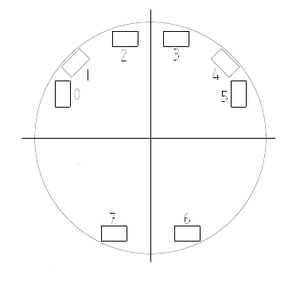
\includegraphics[scale=0.5]{IRSensors}
 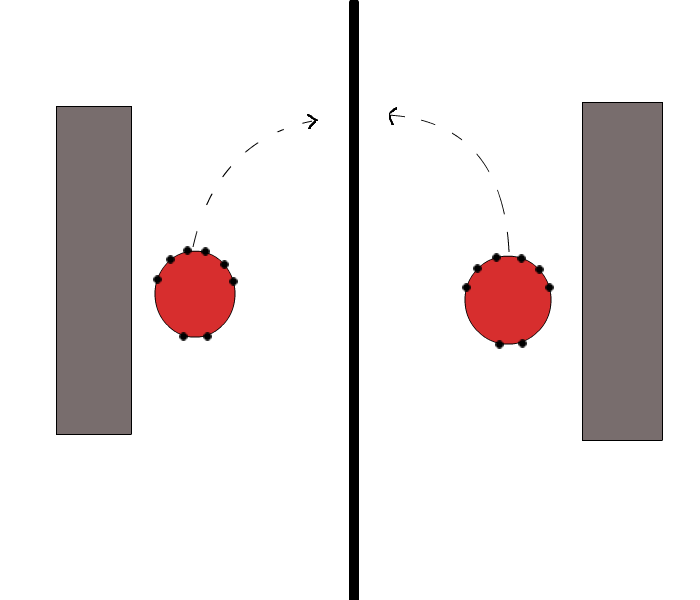
\includegraphics[scale=0.25]{obstacles}
 \centering
 \caption{On the left you can see the positions of the 8 IR sensors in a Khepera robot. On the right, you can see the bahavoiur of our robot near obstacles}
 \end{figure}

\begin{center}
\begin{tabular}{|c|c|}
 \hline
 \textbf{Task} & \textbf{Sensors Used}  \\
 \hline
 Detecting obstacles on left & 0 and 1 \\
 Detecting obstacles on right & 4 and 5 \\
 Detecting obstacles in front & 1, 2, 3, and 4 \\
 \hline
\end{tabular}
\end{center}

\subsection{Food collection}

There are many possible approaches to food collection. One approach is coming back to the nest once the first food item has been found, and simply follow a routine of travelling between these two location. It has the advantage of simplicity and might work very well if a food item is discovered reasonably close to the nest. However, if there is another food item close to the discovered one, it will be ignored in this approach. Therefore, this method is not optimal. The approach in the opposite pole is to continue exploring the arena for food collection, and come back to the nest with all the collected when there is only one minute left. This approach might collect a lot more food than the first one. On the other hand, if the robot does not make it in time, all the effort in food collection goes to waste. As a result, we deicide to choose the approach in between, which is explained in the next paragraph.\\\\
The robot continues to explore for foods until it finds two food sources. Then, it comes back to the nest and drops them off by flashing its LEDs three times. For the rest of its running time, it will use the two previously found food sources to collect food rather than exploring for new ones, as it might take a long time to collect three food items. The routine path is from the nest to the closest food, to the second closest food, and to the nest again. However, if it discovers a new food source on its way back, the two chosen food sources might alter. The robot always chooses the two closest food sources to the nest, thus, if the new discovered food source is closer than one of the other two, it is going to replace the furthest one in the routine path.

\subsection{Navigation}

A*search is an algorithm used to find the shortest route from one point to another on a predefined map. A* calculates the shortest route by calculating a cost for each node. This cost is made up of the distance from the parent node to the node in question and the distance from that node to the goal node. The algorithm keeps track of each node it has chosen along the way so that when it reaches the goal it can look back and return the shortest route. There are two lists of nodes OPEN and CLOSED.  OPEN is the list of aren't nodes of each node chosen, this is used to find the optimal path when you reach the end. CLOSED is the list of paths that have been explored, or contain an object. An overview of the A* algorithm can be observed below:

\begin{enumerate}
 \item Put start node on the list OPEN and calculate cost function of the distance between goal and start
 \item Remove from the list OPEN the node with the smallest cost function and add it to CLOSED. This is the node we choose.
 \item If the chosen node is the goal node then terminate the algorithm and obtain optimal path. Else continue.
 \item Determine all successor nodes of the chosen node and compute the cost function for each of them that are not on the CLOSED list.
 \item Associate with each successor not on list OPEN or CLOSED the cost calculated and put these on the list OPEN.
 \item Associate with any successors already on OPEN the smaller of the cost values just calculated and the previous cost value.
 \item Go to step 2.
\end{enumerate}

\begin{figure}[h]
 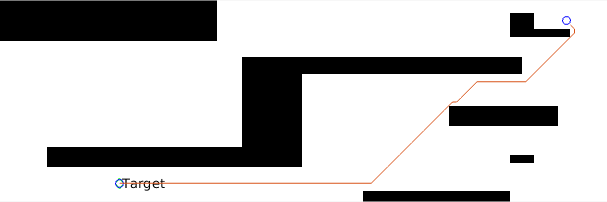
\includegraphics[scale=0.5]{A_1}
 \centering
 \caption{Here is an example of A* algorithm generated on a test map. The two blue points indicates the start and target point, and the green line indicates the optimal path.}
\end{figure}
\begin{center} 
\end{center}
For the A* algorithm to be used we needed to represent the arena in a map format. This was done by taking the image of the map that was provided and manually selecting each object with a black box (see figure 3). We then used image segmentation to convert the image into a binary matrix where a '1' represents an object and a '0' represents empty space.

\begin{figure}[h]
 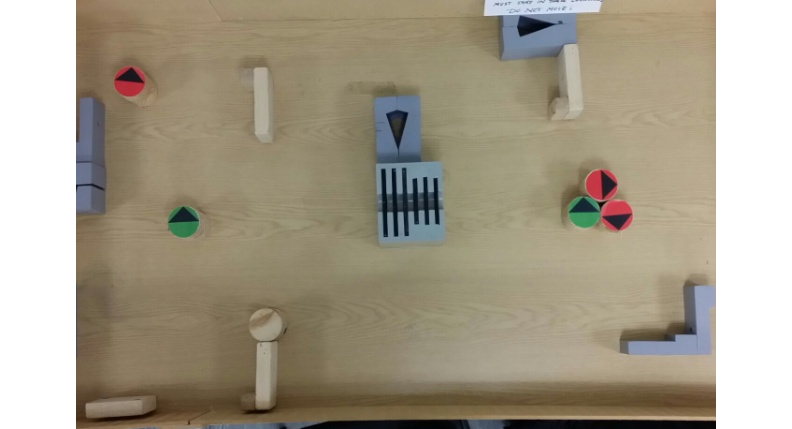
\includegraphics[scale=0.4]{A_2}
 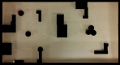
\includegraphics[scale=2.14]{A_3}
 \centering
 \caption{The actual lab environment of the robot, as well as the image used for segmentation with all the obstacles covered in black.}
\end{figure}
\begin{center} 
\end{center}
This gave us a matrix that we could run the A* algorithm on. Initially we attempted to scale the image to the same scale that the robot uses for the x and y co-ordinates it calculates using Odometry. This resulted in an image of around 3000$\times$1400 pixels. Attempting to run the A* algorithm resulted in the program taking a significant amount of time to calculate a route. Thus, in order to solve this problem we ran the algorithm on a scaled down version of the map. Once the optimal route is calculated a set of way-points along the path were stored. These way-points were later scaled up to match the robots Odometry. The resulting map that the A* algorithm was run on was 120$\times$65 pixels (see figure 4). Even on this the algorithm, it took about 15 seconds to find a route from a corner of the map back to the nest. \\\\
Although we implemented the A* algorithm to calculate the optimal path, insufficient time was left to adjust the robots implementation to use these way-points in the practical demo. However, results in the final experiments show that the robot is able follow the way-points (as long as the scale used is correct), and the route that it follows is an efficient route to it's goal.

%Odometery: Correct yourself (postion wise) when you find food for the second time

\section{Results}
%%%%%%%%%%%%%%%%
Our robot is able to explore the arena and receive food signals by a mouse-click on the Odometry graph. It is also able to successfully come back to the nest, as well as indicating it has reached there by flashing its LEDs three times. It continues to search for food, until it finds two food items. After successfully dropping the food items in the nest, it chooses the two closest food it has found so far and it navigates to them in order of their distance to the nest. It does not follow the same path to the food items, but following the most optimal path to the target location using A* search. As explained before, the reason for targeting the two closest food sources rather than the location of the first two food items it finds, is the possibility of discovering new food items on the way back, or going back to one of the previously found food items.\\\\
We did 5 experiments, with each experiment being 5 minutes. We kept the food sources fixed, but we changed the initial angle of the robot in each experiment. A summary of the results can be observed in the table below. The angles is measured with respect to x-axis pointing left. Our robot was able to approximately collect an average of 4.6 each trial. In navigation, A* worked well and our robot's route choices in all 5 experiments seemed to be efficient (see figure 4).

\begin{center}
\begin{tabular}{|c|c|c|c|}
 \hline
  \textbf{Results Table} & \textbf{Initial angle} & \textbf{Total food items collected} & \textbf{Number of crashing in each experiment} \\
 \hline
 experiment 1 & 0 & 4 & 1\\
 experiment 2 & 45 & 6 & 1\\
 experiment 3 & 90 & 2 & 3\\
 experiment 4 & 180 & 6 & 5\\
 experiment 5 & 270 & 5 & 2\\
 \hline
\end{tabular}

\end{center}

A summary of A* path:
\begin{figure}[h]
 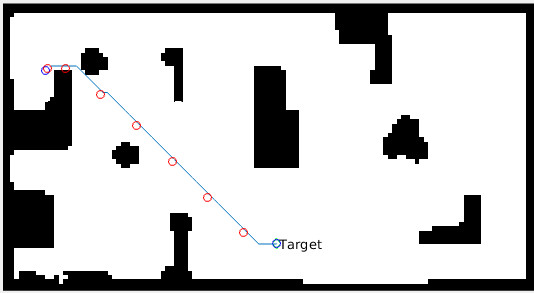
\includegraphics[scale=0.35]{A_4}
 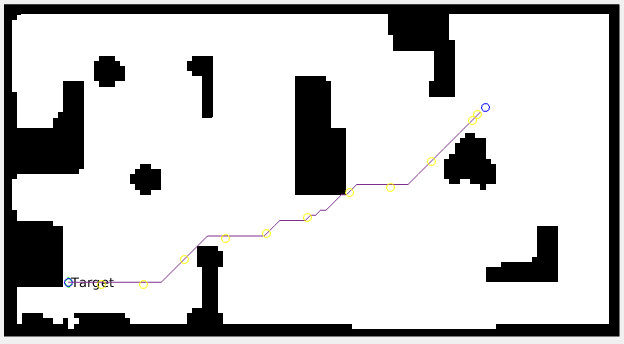
\includegraphics[scale=0.3]{A_5}
 \centering
 \caption{Some examples of A* search tested in the map of the arena.}
\end{figure}
 

\section{Discussion}
%%%%%%%%%%%%%%%%%%%%%%

We have developed an algorithm for a Khepera robot to do exploration, localization, and navigation. Our Khepera robot explores the arena by simply following a straight path, while curving away from the walls and obstacles. It chooses the location of the two closest food items it has found so far, and then follows a direct path to those locations in order of their distance towards nest. It continues to explore until it finds two food items. Our algorithm has done a reasonably good job, and it was able to collect 4 food items within 5 minutes in the practical demo, and winning the competition.  In this section, we analysed our results by indicating some advantages and disadvantages of our approaches, as well as suggesting improvements.

\subsection{Advantages}
 Our algorithm is not as complex as bio-inspired algorithms. However, it has several advantages in comparison to approaches of other teams which we listed below. It is also worth mentioning that the graphs we draw were extremely helpful as visual feedback. Plotting the path of the robot helped us to track the problems very easily, and accelerated the debugging process, both in localization and navigation.
\begin{enumerate}
 \item \textbf{Simplicity}:\\
 One main advantage of our approach is its simplicity. Both the exploration and navigation approaches we used are simple algorithms, and therefore it made it easy and quick for us to debug and track our problems. Complex algorithms such as SLAM are time consuming to implement and difficult to debug. 
 \item \textbf{Reliable Odometry and visual feedback}:
 Another main advantage of our program compare to other teams is very high accuracy in Odometry, even in long runs. We noticed that even after 6 minutes of running, our robot is able to navigate to its desired location with an error of $\pm$10cm. Our robust Odometry in the algorithm comes from two factors:\\
 \begin{enumerate}
  \item First one is taking advantage of the food signals from the demonstrator, and resetting the Odometry when finding food that has been found in the past. Our robot stores the positions of all the foods items it finds in its path. However, if it finds a food item very close to one of stored position of the previously found food items (within 5cm radius), it makes a reasonable assumption of having found the same food source again. Therefore, it resets its position to the position of the close by food item in its memory.
  \item The second factor is adapting the time step in Odometry calculation. The time step we originally used was 0.1 second. But we realized that if we use this value in Odometry calculation, the estimated position is extremely inaccurate. We believe this is the due to the fact that the time between receiving two control commands is not exactly 0.1 second. Therefore, we started changing the value of this parameter to different, but close values. Gradually increasing the $\Delta t$ value (by 0.01s), significant improvement was observed in Odometry. The final value we decided to set $\Delta t$ to was 0.157 second.
 \end{enumerate}
      
 \item \textbf{Randomness in navigation}:\\
  One main issue we observed in our approach (and approaches of other teams) was the robot not being able to find a previously found food item due to Odometry error. Signalling food collection is done by mouse-click, so what if the robot thinks it is in a previously found food source, but the demonstrator is not signalling food collection because the robot is not exactly covering the food item (Odometry error)? As a result, even though our Odometry was highly accurate, we decided to increase the reliability of our food navigation approach by using randomness in movements to avoid this problem. We came up with a fantastic solution.\\\\
  We observed that the error in Odometry occurs in random direction. As a result, we decided to attack this problem using randomness. We increased the error threshold and altered the navigation algorithm for when the robot's position is close to the target food item. If the robot enters in an area within 10cm radius of the target food item, it randomly curves to right and left (with equal probability) until it receives the signal from the demonstrator (see figure 5). This method worked really well, and resulted in never failing at food collection in a previously found food source. It is extremely difficult to achieve 100\% accuracy in Odometry. As a result, coming back to exact same position in long runs is nearly impossible. Random movements in a nearby area until hitting the desired position appeared to be a very good solution. 
 \begin{figure}[h]
 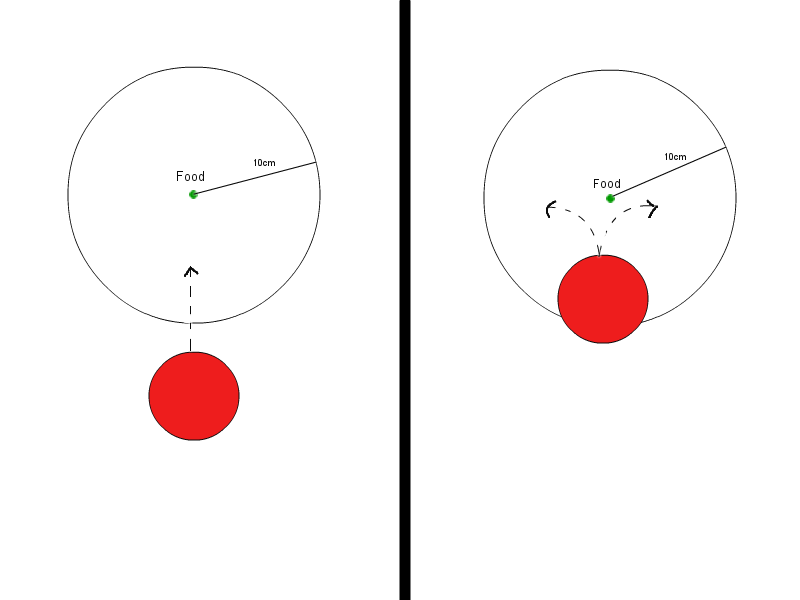
\includegraphics[scale=0.45]{Food_Area}
 \centering
 \caption{If the robot is not within 10cm radius of the food item, it follows a direct path to the food item. Once it finds itself within the area, it randomly curves to left and right (with equal probability), until the demonstrator signals that it hit the food item.}
 \end{figure}
\end{enumerate}


%If we did A*, Add it to methods and use it for exploration. If not, write an advatnage of map independece.
\subsection{Weaknesses and Improvements}
Our algorithm is not optimal and many improvements can be made. There are more optimal and complex algorithms to do this task such as particle filters and SLAM. However, due to insufficient time, and the current algorithm performing reasonably well, we decided to not use them. A summary of the weaknesses and further improvements can be observed below:
\begin{enumerate}
 \item \textbf{Exploration}:\\
 Our Exploration approach has much space for improvements. It is quite low intelligent since it does not have any plan to explore. It also might get stuck in infinite loops in certain situations, such as the situation shown in figure 6. Several improvements can be made such as dividing the map to regions and exploring them one by one, or start exploring the area close to the nest, and gradually increase the exploration area radius.
 \begin{figure}[h]
 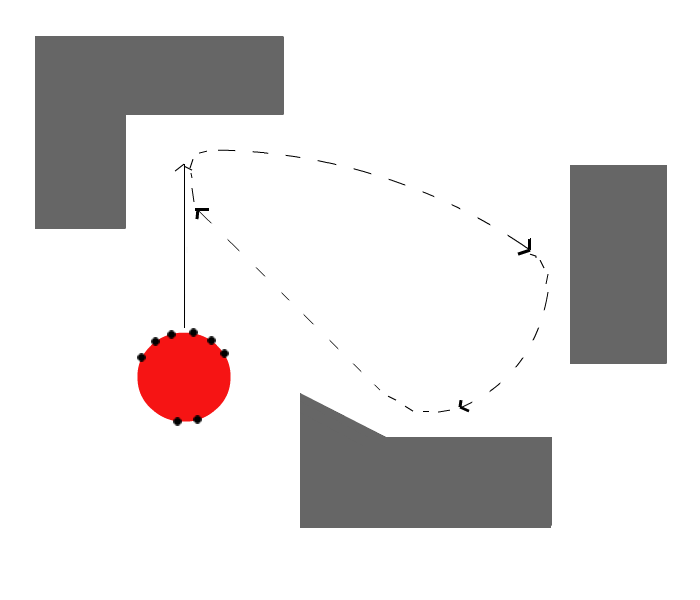
\includegraphics[scale=0.35]{InfiniteLoop}
 \centering
 \caption{A situation that the robot might get stuck in an infinite loop.}
 \end{figure}
 \item \textbf{Food location choices}:\\
 There are certain situations which navigating to the two closest food sources is very inefficient. An example of this can be observed in figure 7. In the situation in figure 7, even if our robot knows about all three food locations, it will ignore the third closest food item and picks up food items 1 and 2 as food choices. However, it can be easily noticed that choosing the food items 1 and 3 is much more efficient. This problem is solvable by adjusting the food collection limits, and allowing collection of more than two food items if there are two food items close to each other. 
 \begin{figure}[h]
 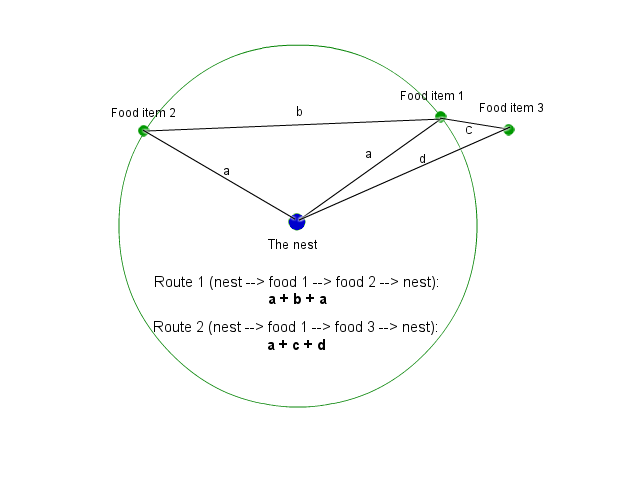
\includegraphics[scale=0.5]{Food_choices}
 \centering
 \caption{In this situation, even though food items 1 and 2 are the closest foods to the nest, it is more optimal to collect the third closest food (number 3) in combination with food item 1. This will result in significant improvement in time for a fixed number of food collection. An even more optimal approach might be to collect all three items before coming to the nest. In other words, adjusting the number of foods to carry home if two of the location are reasonably close to each other.}
 \end{figure}
 \item \textbf{Hardware}:\\
 One of the main difficulties we faced in this task was the occasional crashing during the trials, which made it difficult for us to run long experiments. It was difficult to handle this issue, as it was more of a hardware problem. The approaches we attempted to reduce the crashing was using the mains electricity rather than the battery and holding the connection wire in a comfortable position, which in fact resulted in a better performance.
 
\end{enumerate}

\section{Appendix}
%%%%%%%%%%%%%%%%%%%%%%%

\subsection{Start}
\lstinputlisting[language=Matlab]{../start.m}
\subsection{Main Controller}
\lstinputlisting[language=Matlab]{../robot3_controller.m}
\subsection{Wheels Speed}
\lstinputlisting[language=Matlab]{../wheel_speeds.m}
\subsection{Odometry}
\lstinputlisting[language=Matlab]{../odometery.m}
\subsection{Finding Home}
\lstinputlisting[language=Matlab]{../home_direction.m}
\subsection{Finding Food}
\lstinputlisting[language=Matlab]{../food_direction.m}
\subsection{Food choosing}
\lstinputlisting[language=Matlab]{../food_memory_correction.m}
\subsection{Flash LED}
\lstinputlisting[language=Matlab]{../led_3_times.m}
\end{document}